%--------------------------------------------------------------------
% Reference manual, with description of the options
%--------------------------------------------------------------------
\chapter{Reference manual}
\label{c:3:refman}

We describe \safe commands and their basic usage.

\section{\safe commands}
Each command consists of phases and one can run a \safe command as follows:
\begin{verbatim}
safe {command} [-{option}]*
     [-{phase}:{option}[={input}]]* {filename}+
\end{verbatim}
For example, The command \verb!compile! consists of six phases; 
\verb!parser!, \verb!astRewriter!, and \verb!compiler!.
The following command compiles JavaScript code stored in a file name
``{sample.js}'' located in the current directory without showing detailed
information but printing the result of the \verb!cfgBuilder!
phase into a file name ``{out}'':
\begin{verbatim}
safe analyze -silent
             -cfgBuilder:out=out sample.js
\end{verbatim}

Each phase has its own available options.
The most common options are as follows:
\begin{itemize}
\item \verb!-{phase}:silent!

\safe does not show messages during the phase.

\item \verb!-{phase}:out={string}!

\safe writes the result of the phase to a file \verb!{string}!.
\end{itemize}
and the global options are \verb!-silent! and \verb!-testMode!.

The currently supported commands and their phases are as follows:
\begin{verbatim}
parse          parser
astRewrite     parse >> astRewriter
compile        astRewrite >> compiler
cfgBuild       compile >> cfgBuilder
heapBuild      cfgBuild >> heapBuilder
analyze        heapBuild >> analyzer
bugDetect      analyze >> bugDetector
web            web
help           helper
\end{verbatim}

and phases and their options are as follows:
\begin{itemize}
\item \verb!parser -out={string}!

parses the JavaScript code and generates an Abstract Syntax Tree (AST)
in given files. If multiple files are given, they are concatenated
in the given order before being parsed.

\item \verb!astRewriter -silent!\\
\hspace*{6.3em}\verb!-out={string}!

rewrites a given AST into a simplified AST.

\item \verb!compiler -silent!\\
\hspace*{4.7em}\verb!-out={string}!

generates an Intermediate Representation (IR) from a given AST.

\item \verb!cfgBuilder -silent!\\
\hspace*{5.8em}\verb!-out={string}!

generates a Control Flow Graph (CFG) from a given IR.

\item \verb!heapBuilder -silent!\\
\hspace*{6.3em}\verb!-maxStrSetSize={number}!\\
\hspace*{6.3em}\verb!-aaddrType={string}!\\
\hspace*{6.3em}\verb!-callsiteSensitivity={number}!\\
\hspace*{6.3em}\verb!-loopIter={number}!\\
\hspace*{6.3em}\verb!-loopDepth={number}!\\
\hspace*{6.3em}\verb!-snapshot={string}!\\
\hspace*{6.3em}\verb!-number={string}!\\
\hspace*{6.3em}\verb!-jsModel!

builds initial abstract heap used in the \verb!analyzer! phase
and attaches it into a given CFG.

If \verb!-maxStrSetSize={number}! is given,
the analyzer will use the string set domain with given size limit n.

If \verb!-aaddrType={string}! is given,
the analyzer will use a given address abstraction type;
\verb!"normal"!: allocation-site abstraction and
\verb!"recency"!: recency abstraction with allocation-site abstraction.

If \verb!-callsiteSensitivity={number}! is given,
{number}-depth callsite-sensitive analysis will be executed.

If \verb!-loopIter={number}! is given,
{number}-iteration loop-sensitive analysis will be executed.

If \verb!-loopDepth={number}! is given,
{number}-depth loop-sensitive analysis will be executed.

If \verb!-snapshot={string}! is given,
analysis with an initial heap generated from a dynamic snapshot(*.json)
will be executed.

If \verb!-jsModel! is given,
analysis with JavaScript models will be executed.

\item \verb!analyzer -silent!\\
\hspace*{4.7em}\verb!-console!\\
\hspace*{4.7em}\verb!-exitDump!\\
\hspace*{4.7em}\verb!-out={string}!

analyzes the given CFG with the given initial abstract heap.

If \verb!-console! is given,
a user can debug analysis results by investigating the intermediate
status of the analysis.

If \verb!-exitDump! is given,
it shows the abstract state of the top-level exit node.

\item \verb!bugDetector -silent!

detects possible bugs in a given analysis result.

\item \verb!web -port={number}!

allows a user to investigate the analysis status from a browser
based on network connection. It starts web server with the given
port number (default: 8080). We describe this in Section~\ref{s:3:2:2:refman}

\item \verb!help!

shows the usage of \safe commands to the standard output.
\end{itemize}

\medskip
The \verb!parser! phase parses the JavaScript code in a given file and
rewrites obvious dynamic code generation into other statements without using
dynamic code generation but with the same semantics.  For example, the following
JavaScript code
\begin{verbatim}
function f() { return 3; }
eval("f()")
\end{verbatim}
is rewritten as follows:
\begin{verbatim}
function f() { return 3; }
f();
\end{verbatim}

\medskip
The \verb!astRewriter! phase rewrites its AST representation into a simpler AST
using three kinds of AST transformations:
\begin{itemize}
\item \verb!Hoister! lifts the declarations of functions and variables inside
programs and functions up to the beginning of them.
\item \verb!Disambiguator! checks some static restrictions and renames identifiers
to unique names.
\item \verb!WithRewriter! rewrites the \verb!with! statements that do not include
any dynamic code generation such as \verb!eval! into other statements without using
the \verb!with! statement but with the same semantics~\cite{dls13,withtr}.
\end{itemize}

% Note that building a graph visualization format of CFGs requires the \verb!dot! program
% from Graphviz~\cite{graphviz} be in your path.
% For example, the following command:
% \begin{verbatim}
% safe cfgBuild -cfgBuilder:dot=dot sample.js
% \end{verbatim}
% runs the following command:
% \begin{verbatim}
% dot -Tpdf dot.gv -o dot.pdf
% \end{verbatim}
% to produce something like the following:
% \begin{figure}[H]
% 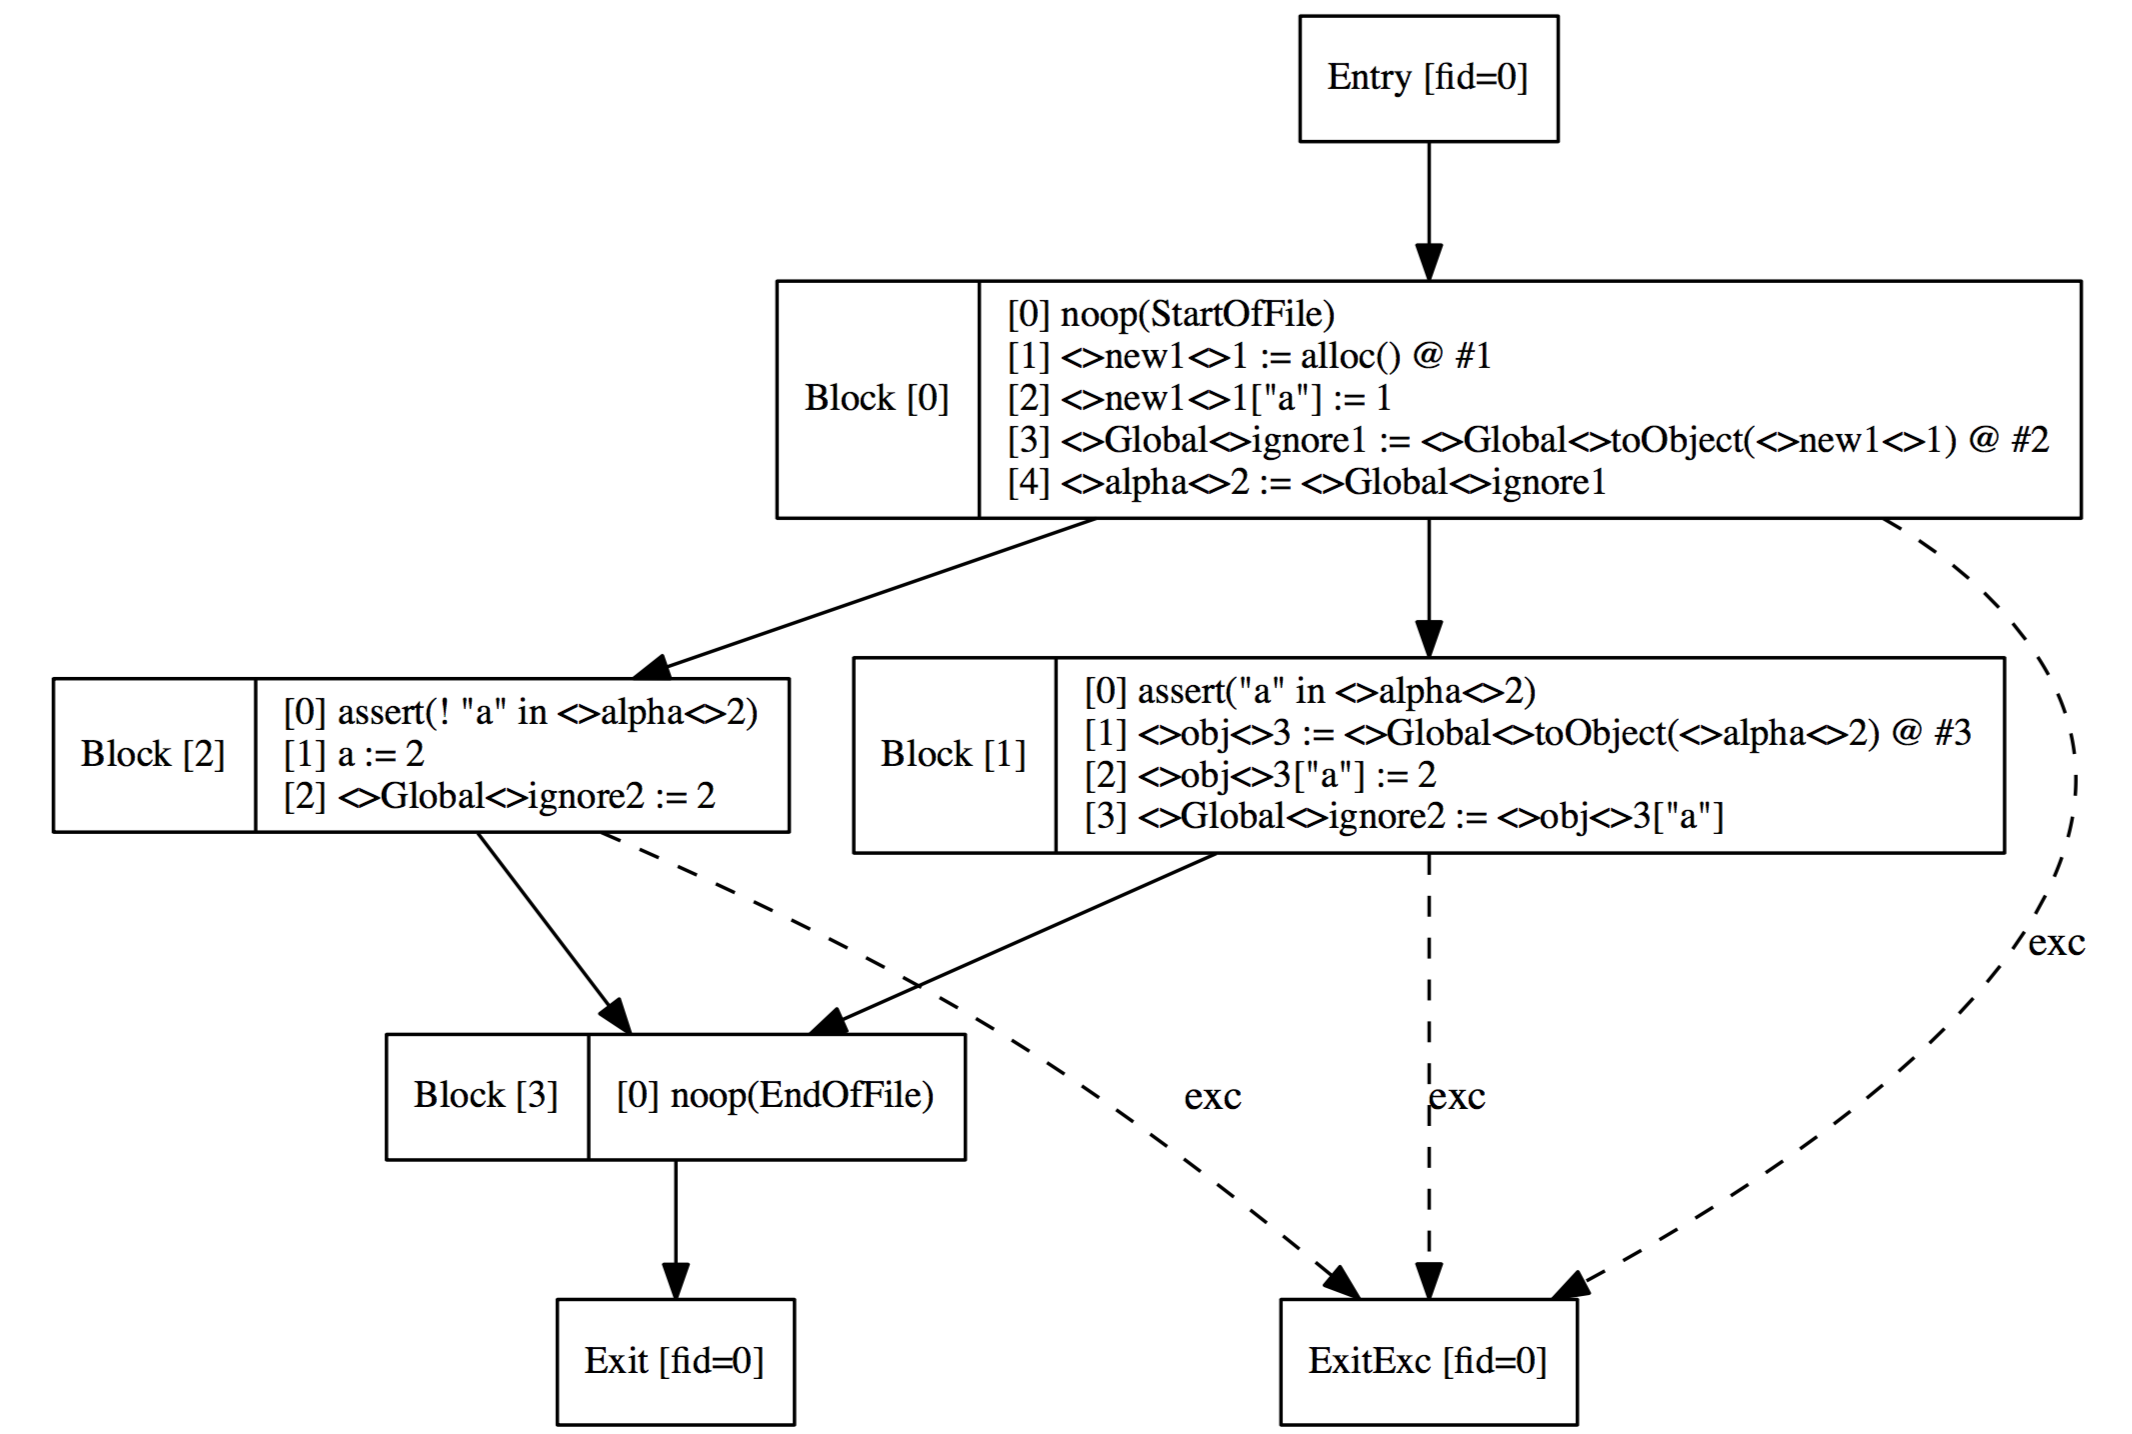
\includegraphics[width=8.75cm]{cfg.png}
% \end{figure}

\section{\safe analyzer debugging}
When the \verb!-analyzer:console! option is given to the \texttt{analyze} command,
\safe provides a REPL-style console debugger.
For example, the following command:
\begin{verbatim}
safe analyze -analyzer:console test.js
\end{verbatim}
shows the list of available commands for debugging and
the starting point of the analysis:
{\small
\begin{verbatim}
Command list:
- help
- next           jump to the next iteration. (same as "")
- jump           Continue to analyze until the given
                 iteration.
- print          Print out various information.
- result         Print out various information.
- run_insts      Run instruction by instruction.
- move           Change a current position.
- home           Reset the current position.
- run            Run until meet some break point.
- break          Add a break point.
- break-list     Show the list of break points.
- break-rm       Remove a break point.
- find-bot       Find the instruction whose result is
                 bottom.
- restart        Restart the analysis.
For more information, see 'help <command>'.

<top-level[0]: Entry[-1], NoLoop> @sample.js:1:1
 Iter[0] >
\end{verbatim}
}

The current status is denoted as follows:
{\small
\begin{verbatim}
<{fun-name}[{fid}]: {block-kind}[{bid}],
 {sensitivity}> @{filename}:{span}
Iter[{#iteration}] >
\end{verbatim}
}
\noindent
where \verb!fun-name! and \verb!fid! are the name and the id of the current function,
respectively, \verb!block-kind! and \verb!bid!
are the kind and the id of the current block, respectively,
\verb!sensitivity! is the sensitivity of the current analysis,
\verb!filename! is the name of the file being analyzed,
\verb!span! is the location of the current analysis, and
\verb!#iteration! is the iteration number of the current analysis.
We support call-context sensitivity based on call-sites
and loop sensitivity based on loop iterations and inner-loop depths
as analysis sensitivities.

A block is one of the following kinds:
\begin{itemize}
\itemsep-.1em
\item Entry: the entry block of a function
\item Exit: the exit block of a function
\item ExitExc: a block denoting uncaught exceptions in a function
\item Call: a block denoting a function call
\item AfterCall: a block receiving a return value of a function call
\item AfterCatch: a block receiving uncaught exceptions after a function call
\item Block: a normal block with instructions
\item LoopHead: a block denoting a loop head
\item LBreak: a block right after the \verb!break! statement
\item LCont: a block right after the \verb!continue! statement
\item Branch: a block denoting a branch
\item Switch: a block denoting a head of \verb!switch! statement
\item Case: a block denoting a \verb!case! clause in a \verb!switch! statement
\item Default: a block denoting the \verb!default! clause
  in a \verb!switch! statement
\item Try: a block denoting a head of \verb!try! block
\item Finally: a block denoting a \verb!finally! block
\item Catch: a block denoting a \verb!catch! block
\item Label({string}): a block denoting a user label \verb!{string}!
\item ModelBlock: a block denoting a modeled function
\end{itemize}

The \verb!help! command displays a list of available commands and
the \verb!help <command>! command displays the usage of the \verb!<command>!.
For example:
{\small
\begin{verbatim}
<function[0] top-level: Entry[-1], ()> @test.js:1:1
Iter[0] > help print
usage: print state(-all) ({keyword})
       print heap(-all) ({keyword})
       print context ({keyword})
       print block ({fid}:{bid})
       print loc {LocName} ({keyword})
       print func ({fid})
       print function ({fid})
       print worklist
       print ipsucc
       print trace
\end{verbatim}
}
\noindent
shows the usage of the \verb!print! command.

\medskip
The \verb!next! command proceeds the analysis of the current block,
which is the default command.  For example:
{\small
\begin{verbatim}
<top-level[0]: Entry[-1], NoLoop> @test.js:1:1
 Iter[0] >

<top-level[0]: Block[0], NoLoop> @test.js:2:1-8:20
\end{verbatim}
}

\medskip
The \verb!jump {#iteration}! command proceeds the analysis until the given
number of iterations.  For example:
{\small
\begin{verbatim}
<top-level[0]: Entry[-1], NoLoop> @test.js:1:1
 Iter[0] > jump 10

<f[1]: Block[4], NoLoop> @test.js:5:8-19
 Iter[10] >
\end{verbatim}
}

\medskip
The \verb!print! command displays the status just before
analyzing the current block.  We describe it in Section~\ref{s:3:2:1:refman}.

\medskip
The \verb!result! command displays the status after analyzing
the current block:
\begin{itemize}
\item \verb!result (exc-)state(-all) ({keyword})!

It displays the state in the same way as the \verb!print! command does,
and it can additionally show the exception state generated after the analysis.
\item \verb!result (exc-)loc {LocName}!

It finds and displays the location in the same way as the \verb!print! command does,
and it can additionally find and display the location from
the exception state generated after the analysis.
\end{itemize}

\medskip
The \verb!run_insts! command shows the list of instructions in the current block,
and it enables to analyze each instruction.  It opens a sub-console, which provides 3 kinds
of commands:
\begin{itemize}
\itemsep-.1em
\item \verb!s! shows the state
\item \verb!q! quits the analysis
\item \verb!n! analyzes the next instruction; the default command
\end{itemize}
For example:
{\small
\begin{verbatim}
<top-level[0]: Block[0], NoLoop> @test.js:2:1-8:20
 Iter[1] > run_insts
Block[0] -> [1], ExitExc
  [0] f := function (1) @ #6, #7
  [1] noop(StartOfFile)
  [2] x := 1
  [3] <>obj<>9 := @ToObject(f) @ #8
  [4] <>arguments<>10 := allocArg(0) @ #9
  [5] <>fun<>11 := @GetBase(f)
  [6] <>this<> := enterCode(<>fun<>11)

inst: [0] f := function (1) @ #6, #7
('s': state / 'q': stop / 'n','': next)
>

inst: [1] noop(StartOfFile)
('s': state / 'q': stop / 'n','': next)
>
\end{verbatim}
}

\medskip
The \verb!move {fid}:{{bid}|entry|exit|exitExc}! command
moves the current block to the given block denoted by the id of a function,
the id of a block, and the kind of the block.  For example:
{\small
\begin{verbatim}
<top-level[0]: Block[0], NoLoop> @test.js:2:1-8:20
 Iter[1] > move 0:entry
* current control point changed.

<top-level[0]: Entry[-1], NoLoop> @test.js:1:1
 Iter[1] >
\end{verbatim}
}

\medskip
The \verb!home! command moves the current block back to the original
block to be analyzed.  For example:
{\small
\begin{verbatim}
<top-level[0]: Entry[-1], NoLoop> @test.js:1:1
 Iter[1] > home
* reset the current control point.

<top-level[0]: Block[0], NoLoop> @test.js:2:1-8:20
 Iter[1] >
\end{verbatim}
}

\medskip
The \verb!run! command proceeds the analysis until encountering a break
point.  A short-key for this command is Ctrl-d.  For example:
{\small
\begin{verbatim}
<top-level[0]: Entry[-1], NoLoop> @test.js:1:1
 Iter[0] > break 0:exit

<top-level[0]: Entry[-1], NoLoop> @test.js:1:1
 Iter[0] > run

<top-level[0]: Exit[-2], NoLoop> @test.js:10:1
 Iter[14] >
\end{verbatim}
}

\medskip
The \verb!break! command sets up a break point at the given block.
For example:
{\small
\begin{verbatim}
<top-level[0]: Entry[-1], NoLoop> @test.js:1:1
 Iter[0] > break 0:exit

<top-level[0]: Entry[-1], NoLoop> @test.js:1:1
 Iter[0] > run

<top-level[0]: Exit[-2], NoLoop> @test.js:10:1
 Iter[14] >
\end{verbatim}
}

\medskip
The \verb!break-list! command shows a list of blocks with
break points.  For example:
{\small
\begin{verbatim}
top-level[0]: Exit[-2], NoLoop> @test.js:10:1
 Iter[14] > break-list
* 1 break point(s).
  [0] function[0] Exit[-2]

<top-level[0]: Exit[-2], NoLoop> @test.js:10:1
 Iter[14] >
\end{verbatim}
}

\medskip
The \verb!break-rm {break-order}! command
removes the break point of a given block
denoted by the order in the result of \verb!break-list!.
For example:
{\small
\begin{verbatim}
<top-level[0]: Exit[-2], NoLoop> @test.js:10:1
 Iter[14] > break-list
* 1 break point(s).
  [0] function[0] Exit[-2]

<top-level[0]: Exit[-2], NoLoop> @test.js:10:1
 Iter[14] > break-rm 0
* break-point[0] removed.
[0] function[0] Exit[-2]

<top-level[0]: Exit[-2], NoLoop> @test.js:10:1
 Iter[14] > break-list
* no break point.

<top-level[0]: Exit[-2], NoLoop> @test.js:10:1
 Iter[14] >
\end{verbatim}
}

\medskip
The \verb!find-bot! command finds the instruction
that generates the bottom abstract state.  For example:
{\small
\begin{verbatim}
<top-level[0]: Block[2], NoLoop> @branch.js:2:5-12
 Iter[3] > find-bot
The result of the following instruction is bottom:
  [0] assert(x !== 0)

<top-level[0]: Block[2], NoLoop> @branch.js:2:5-12
 Iter[3] >
\end{verbatim}
}

\medskip
The \verb!restart! command restarts the analysis.  For example:
{\small
\begin{verbatim}
<top-level[0]: Exit[-2], NoLoop> @test.js:10:1
 Iter[14] > restart

<top-level[0]: Entry[-1], NoLoop> @test.js:1:1
 Iter[0] >
\end{verbatim}
}

\subsection{Analyzer debugging with printing}
\label{s:3:2:1:refman}
The \verb!print! command displays the status just before
analyzing the current block.

\medskip\noindent
\fbox{\texttt{print state(-all) (\{keyword\})}}\\[.2em]
The \verb!print state! command displays the current state,
and the \verb!print state-all! command
displays the current state including all system addresses.
When a keyword is given, it displays only the parts that include the keyword.
For example:
{\small
\begin{verbatim}
<top-level[0]: Exit[-2], NoLoop> @test.js:31:1
 Iter[15] > print state result
            __result1 -!> [ttf] UInt
            __result2 -!> [ttf] UInt
            __result3 -!> [ttf] UInt
\end{verbatim}
}

\medskip\noindent
\fbox{\texttt{print heap(-all) (\{keyword\})}}\\[.2em]
The \verb!print heap! command displays the heap of the current state
in the same way as \verb!print state!.

\medskip\noindent
\fbox{\texttt{print context(-all) (\{keyword\})}}\\[.2em]
The \verb!print heap! command displays the context of the current state
in the same way as \verb!print state!.

\medskip\noindent
\fbox{\texttt{print block (\{fid\}\{bid\})}}\\[.2em]
The \verb!print block! command displays the information of
the current block. For example:
{\small
\begin{verbatim}
<top-level[0]: Block[0], NoLoop> @test.js:2:1-10:20
 Iter[1] > print block
span: test.js:2:1-10:20
Block[0] -> [1], ExitExc
  [0] f := function (1) @ #6, #7
  [1] noop(StartOfFile)
  [2] x := 1
  [3] <>obj<>9 := @ToObject(f) @ #8
  [4] <>arguments<>10 := allocArg(0) @ #9
  [5] <>fun<>11 := @GetBase(f)
  [6] <>this<> := enterCode(<>fun<>11)
\end{verbatim}
}

Moreover, it displays the information of the given block denoted
by the id of a function, and the id or the kind of the block.
For example:

{\small
\begin{verbatim}
<top-level[0]: Block[0], NoLoop> @test.js:2:1-10:20
 Iter[1] > print block 1:0
span: test.js:4:8-5:19
Block[0] -> [1], ExitExc
  [0] <>ff<>1 := function (2) @ #1, #2
  [1] <>x<>2 := 2
  [2] <>obj<>5 := @ToObject(<>ff<>1) @ #3
  [3] <>arguments<>6 := allocArg(0) @ #4
  [4] <>fun<>7 := @GetBase(<>ff<>1)
  [5] <>this<> := enterCode(<>fun<>7)
\end{verbatim}
}

\medskip\noindent
\fbox{\texttt{print loc \{LocName\} (\{keyword\})}}\\[.2em]
The \verb!print loc {LocName}! command shows the object
bound at a given location in the current state.
When a keyword is given, it displays only the parts that include the keyword
in the object.  For example:
{\small
\begin{verbatim}
<top-level[0]: Exit[-2], NoLoop> @test.js:2:1
 Iter[2] > print loc R#1
R#1 -> Internal Properties:
       [[Class]] -!> "Object"
       [[Extensible]] -!> true
       [[Prototype]] -!> R#Object.prototype
       DEFAULT: (⊥Elem, Top(absent))
       Normal Properties:
       DEFAULT: (⊥DataProp, Top(absent))
\end{verbatim}
}

\medskip\noindent
\fbox{\texttt{print func (\{fid\})}}\\[.2em]
It displays the list of functions.
If a function id is given, it displays the name and the span of it.
For example:
{\small
\begin{verbatim}
<top-level[0]: Entry[-1], NoLoop> @test.js:1:1
 Iter[0] > print func 1
* function name: f
* span info.   : test.js:1:1-15
\end{verbatim}
}

\medskip\noindent
\fbox{\texttt{print function (\{fid\})}}\\[.2em]
It displays the detailed control flows in the current function.
If a function id is given, it displays that of the corresponding function.
For example:
{\small
\begin{verbatim}
<top-level[0]: Entry[-1], NoLoop> @test.js:1:1
 Iter[0] > print function 1
function[1] f {
  Entry[-1] -> [0]

  Block[0] -> Exit, ExitExc
    [0] x := 1

  Exit[-2]

  ExitExc[-3]

}
\end{verbatim}
}

\medskip\noindent
\fbox{\texttt{print worklist}}\\[.2em]
It shows the work in the current worklist.  For example:
{\small
\begin{verbatim}
<top-level[0]: Block[1], NoCall x NoLoop> @test.js:0:0
 Iter[2] > print worklist
* Worklist set
(0:Block[1], NoCall x NoLoop)
(0:Block[2], NoCall x NoLoop)
\end{verbatim}
}

\medskip\noindent
\fbox{\texttt{print ipsucc}}\\[.2em]
It displays the information of the current inter-procedural successor.
For example:
{\small
\begin{verbatim}
<f[1]: Exit[-2], NoLoop> @test.js:1:15
 Iter[17] > print ipsucc
* successor map
- src: (1:Exit[-2], NoLoop)
- dst:
  (0:AfterCall[2], NoLoop), mayOld: (#4, #1, #5, #2),
    mustOld: (#4, #1, #5, #2)
  (0:AfterCall[6], NoLoop), mayOld: (#4, #7, #1, #5,
    #8, #2), mustOld: (#4, #7, #1, #5, #8, #2)
\end{verbatim}
}

\subsection{Analyzer debugging with browsing}
\label{s:3:2:2:refman}
The \verb!safe web! command starts a web server to allows
users to investigate the analysis status from a browser.
Consider the following snapshot:
\begin{figure}[H]
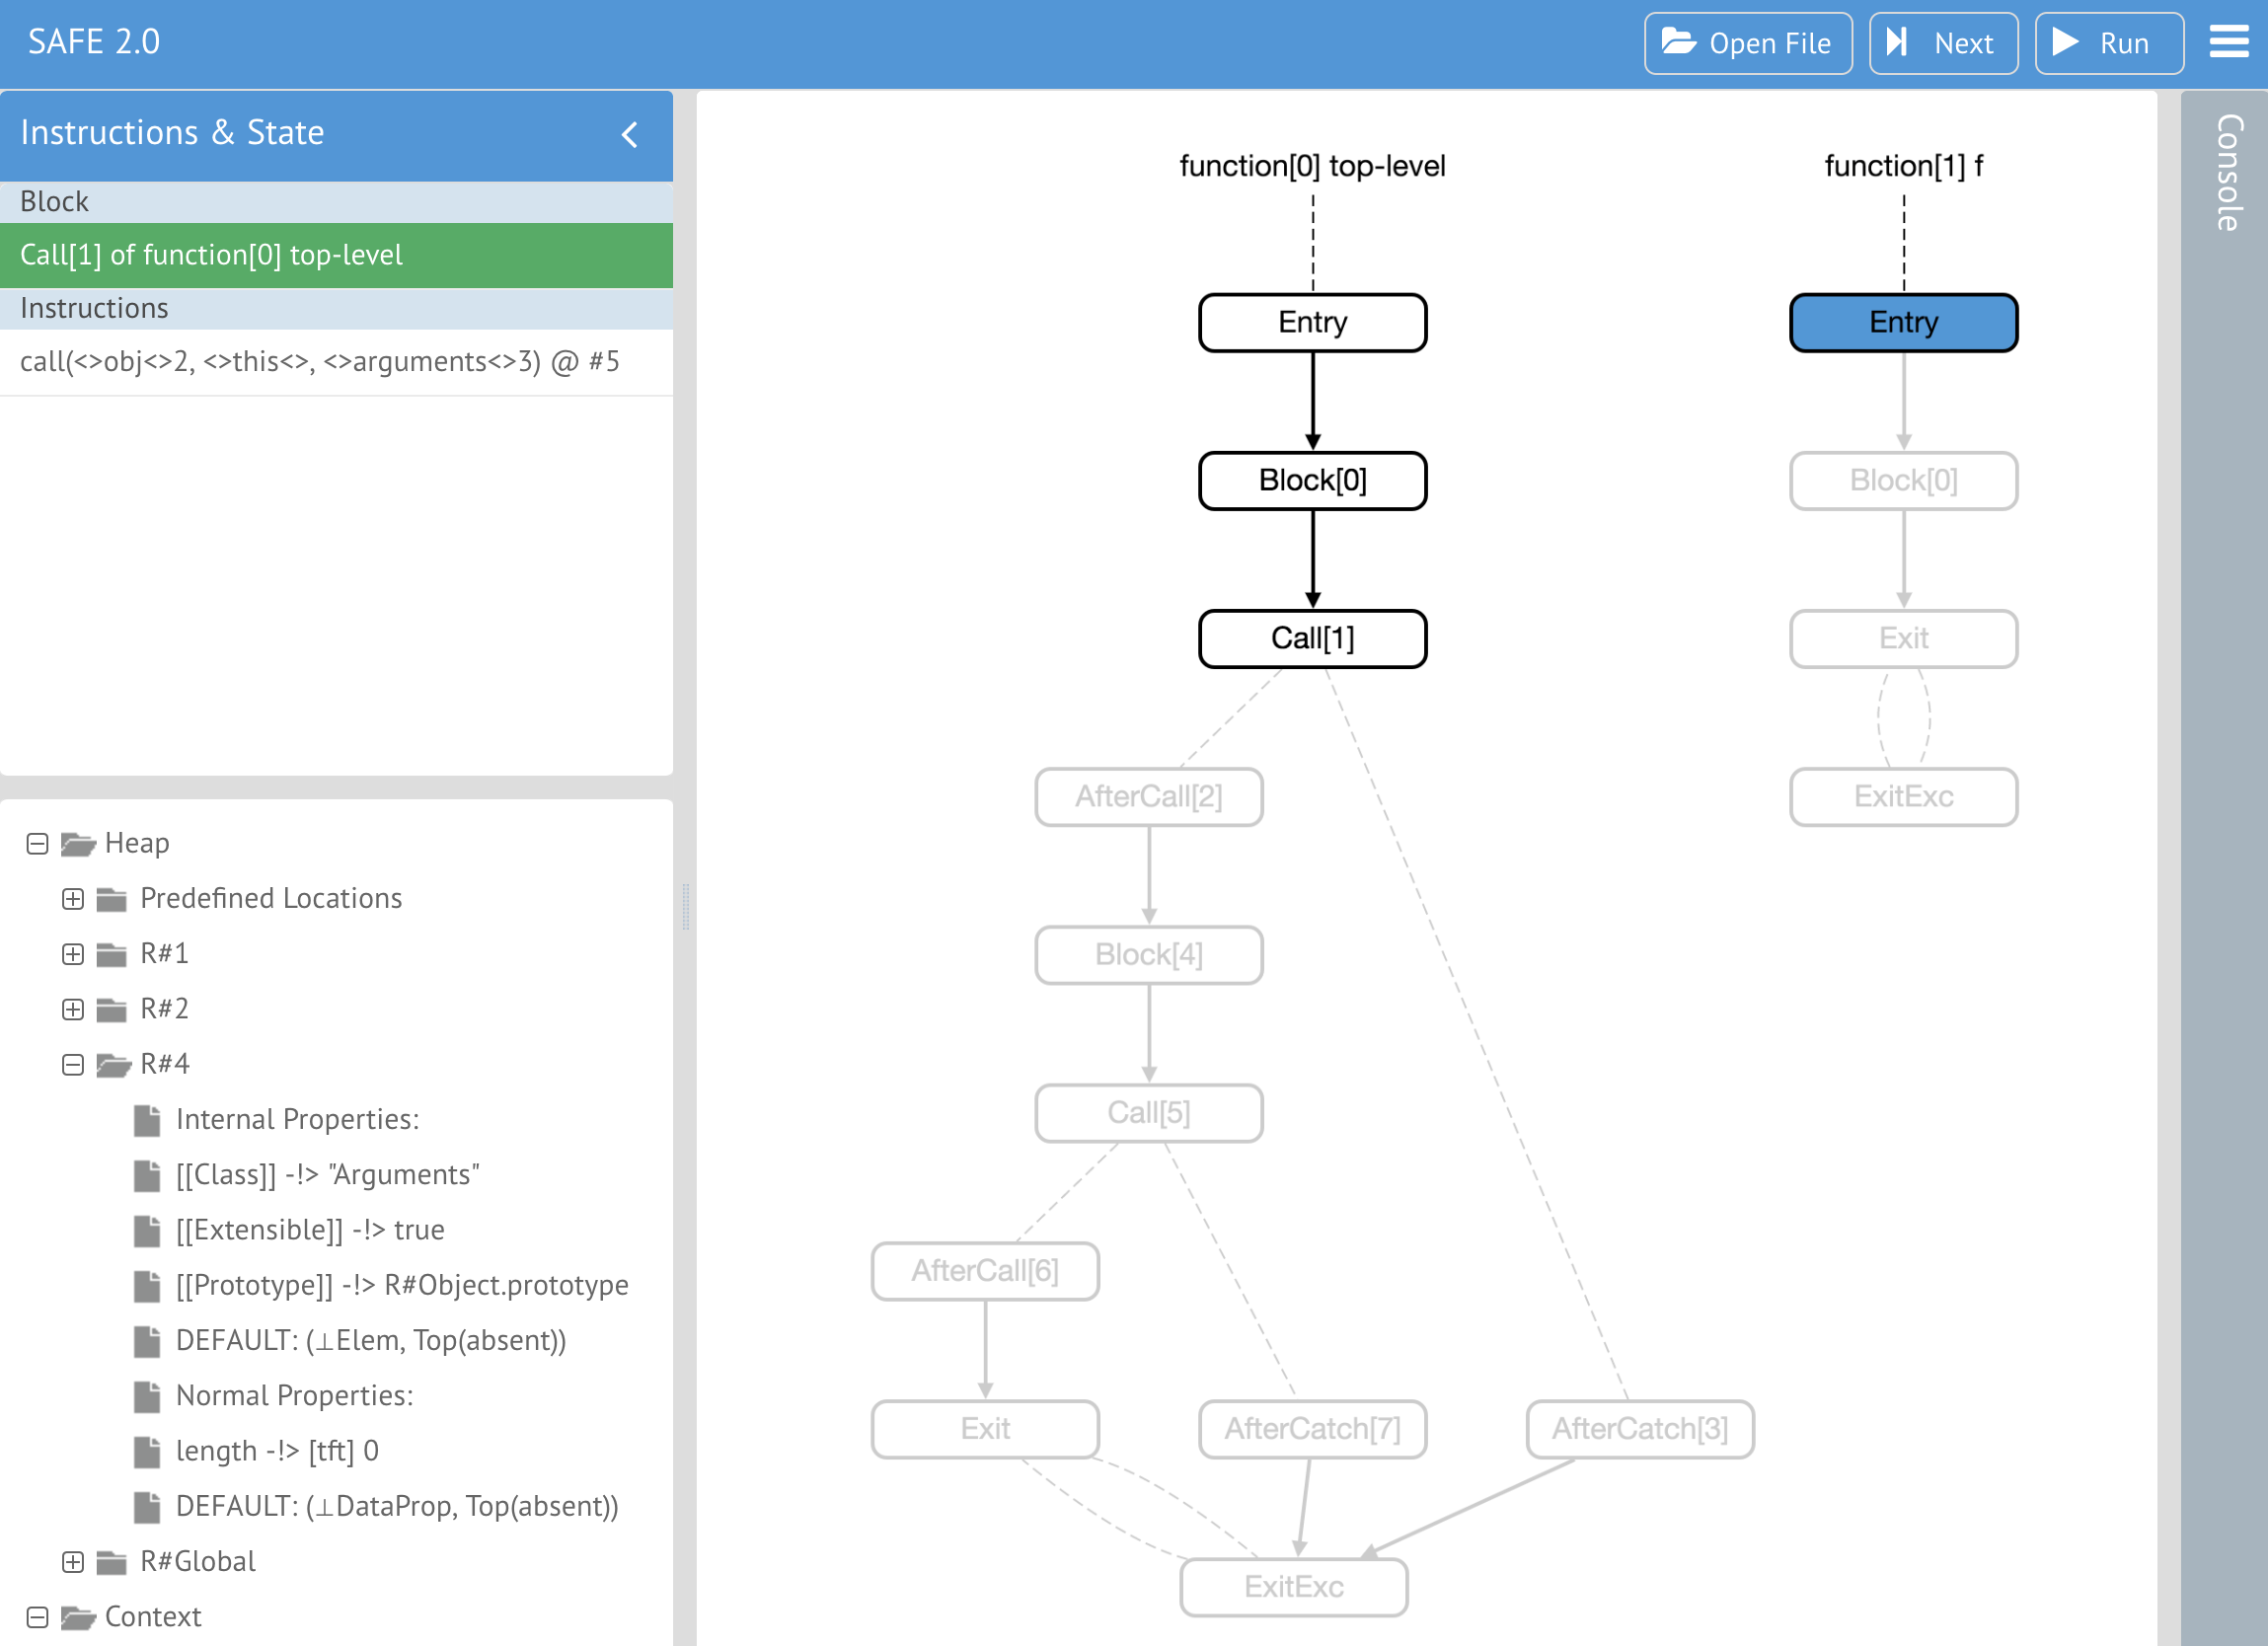
\includegraphics[width=8.75cm]{htmldebugger.png}
\end{figure}
\noindent
which shows the current CFG in the middle.
Nodes in black lines denote the blocks that are analyzed,
those in gray lines denote the blocks not yet being analyzed, and
colored nodes denote the blocks that are currently in the worklist of the analyzer.
One can toggle whether to show the nodes in the worklist by the menu button on the top right.
When a user selects a block from the CFG, the list of the instructions in the block
and the state just before analyzing the block are displayed on the left.
Moreover, users can use all functionalities of the console debugger
through the console screen in the right side.
